% topic3.tex -- Topic 3: Motion in gravitational fields, Questions 49-72.
% (New questions; they do not repeat the 30 in output/M5T3_Gravity_MC_Quiz.pdf.)
\topictitle{Topic 3 - Motion in Gravitational Fields}

% ---- Q49 (Newton's third law)
\begin{quizq}{}
Two objects, of mass $m$ and $4m$, are a distance $d$ apart. The gravitational force on the $4m$
object due to the $m$ object is $F$.

What is the size of the gravitational force on the $m$ object due to the $4m$ object?
\opts{$\dfrac{F}{4}$}{$F$}{$4F$}{$16F$}
\end{quizq}

% ---- Q50 (g from mass and radius ratios)
\Needspace{12\baselineskip}
\begin{quizq}{}
A planet has 5 times the mass of Earth and 2.5 times the radius of Earth.

What is the magnitude of the gravitational field strength close to the surface of the planet?
\opts{$0.8\,g$}{$2.0\,g$}{$5.0\,g$}{$31\,g$}
\end{quizq}

% ---- Q51 (force when one mass doubles and the distance triples)
\Needspace{12\baselineskip}
\begin{quizq}{}
The gravitational force between two objects is $F$. The mass of one object is doubled, and the
distance between them is tripled.

What is the new gravitational force?
\opts{$\dfrac{2F}{9}$}{$\dfrac{2F}{3}$}{$6F$}{$18F$}
\end{quizq}

% ---- Q52 (g at an altitude of 1000 km)
\Needspace{11\baselineskip}
\begin{quizq}{}
What is the gravitational field strength at an altitude of \qty{1000}{km} above Earth's surface?
\opts{\qty{7.4}{N.kg^{-1}}}{\qty{8.5}{N.kg^{-1}}}{\qty{400}{N.kg^{-1}}}{\qty{5.4e7}{N.kg^{-1}}}
\end{quizq}

% ---- Q53 (graph of orbital speed against radius)
\Needspace{30\baselineskip}
\begin{quizq}{}
Satellites move in circular orbits of different radii, $r$, around the same planet.

Which graph best shows the orbital speed, $v$, of the satellites against $r$?
\gridopts{%
  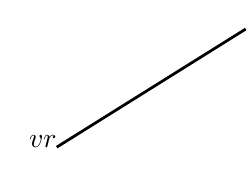
\begin{tikzpicture}\gaxesP{$v$}{$r$}
    \draw[line width=1pt] (0,0) -- (2.4,1.5);
  \end{tikzpicture}}
  {%
  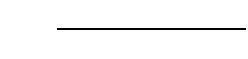
\begin{tikzpicture}\gaxesP{$v$}{$r$}
    \draw[line width=1pt] (0,0.9) -- (2.4,0.9);
  \end{tikzpicture}}
  {%
  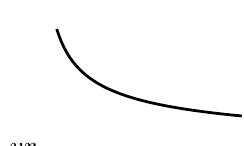
\begin{tikzpicture}\gaxesP{$v$}{$r$}
    \draw[line width=1pt, domain=0.25:2.6, samples=50, smooth] plot (\x, {0.8/sqrt(\x)});
  \end{tikzpicture}}
  {%
  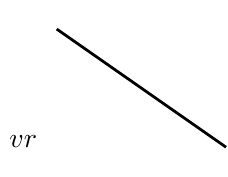
\begin{tikzpicture}\gaxesP{$v$}{$r$}
    \draw[line width=1pt] (0.25,1.5) -- (2.4,0);
  \end{tikzpicture}}
\end{quizq}

% ---- Q54 (Kepler's third law: Mars)
\Needspace{13\baselineskip}
\begin{quizq}{}
Mars orbits the Sun with a period of 1.88 years.

The average distance from the Sun to Earth is one astronomical unit.

What is the average distance between Mars and the Sun in astronomical units?
\opts{1.23}{1.37}{1.52}{2.58}
\end{quizq}

% ---- Q55 (period of a satellite at 800 km)
\Needspace{11\baselineskip}
\begin{quizq}{}
A satellite is in a circular orbit at an altitude of \qty{800}{km} above Earth's surface. What is
its orbital period?
\opts{3.7 minutes}{84 minutes}{101 minutes}{\num{6.1e5} minutes}
\end{quizq}

% ---- Q56 (uses of LEO and GEO)
\Needspace{18\baselineskip}
\begin{quizq}{}
Some satellites must watch one region of Earth all the time. Others take very detailed photographs
of Earth's surface. Which statement correctly explains the choice of orbit?
\opts{Geostationary satellites stay above one point, so they can watch one region all the time.
   Low Earth orbit satellites are closer, so they can take more detailed photographs.}
  {Geostationary satellites are closer to Earth, so they can take more detailed photographs.}
  {Low Earth orbit satellites stay above one point on Earth, so they can watch one region all the
   time.}
  {Low Earth orbit and geostationary satellites have the same period, but different altitudes.}
\end{quizq}

% ---- Q57 (Kepler's laws)
\Needspace{15\baselineskip}
\begin{quizq}{}
Which statement is a correct statement of one of Kepler's laws of planetary motion?
\opts{Each planet moves in a circle with the Sun at the centre.}
  {Each planet moves at a constant speed around the Sun.}
  {For all the planets, the square of the period is proportional to the cube of the average
   distance from the Sun.}
  {For all the planets, the square of the period is proportional to the mass of the planet.}
\end{quizq}

% ---- Q58 (direction of the gravitational force in an elliptical orbit)
% S at E = 120 deg on the ellipse (3cosE, 1.8sinE); Earth at the focus (2.4, 0).
\Needspace{30\baselineskip}
\begin{quizq}{}
A satellite moves anticlockwise in an elliptical orbit around Earth. The cross marks the centre of
the ellipse.
\begin{center}
  \begin{tikzpicture}[scale=1.3]
    \draw[line width=0.7pt] (0,0) ellipse (3 and 1.8);
    \draw[->, line width=0.7pt] (0.35,1.8) -- (-0.35,1.8);
    \shade[ball color=black!25] (2.4,0) circle (0.35); \node[below=8pt, font=\small] at (2.4,0) {Earth};
    \draw (-0.1,-0.1) -- (0.1,0.1); \draw (-0.1,0.1) -- (0.1,-0.1);
    \coordinate (S) at (-1.5,1.559);
    \draw[force] (S) -- ++(-1.04,-0.36) node[left, font=\small\bfseries] {A};
    \draw[force] (S) -- ++(0.762,-0.793) node[below right=-1pt, font=\small\bfseries] {B};
    \draw[force] (S) -- ++(0.36,-1.04) node[below, font=\small\bfseries] {C};
    \draw[force] (S) -- ++(1.02,-0.408) node[right, font=\small\bfseries] {D};
    \draw[fill=white] ($(S)+(-0.12,-0.07)$) rectangle ($(S)+(0.12,0.07)$);
  \end{tikzpicture}
\end{center}
Which arrow shows the direction of the gravitational force on the satellite at the position shown?
\opts{$A$}{$B$}{$C$}{$D$}
\end{quizq}

% ---- Q59 (mass of Saturn from Titan)
\Needspace{12\baselineskip}
\begin{quizq}{}
Titan, a moon of Saturn, has a nearly circular orbit of radius \qty{1.22e9}{m} and an orbital period
of \qty{1.38e6}{s}. What is the mass of Saturn?
\opts{\qty{4.6e17}{kg}}{\qty{1.4e25}{kg}}{\qty{5.6e26}{kg}}{\qty{7.8e32}{kg}}
\end{quizq}

% ---- Q60 (weight at an altitude of 3 Earth radii)
\Needspace{12\baselineskip}
\begin{quizq}{}
An astronaut weighs \qty{800}{N} on Earth's surface. What is the gravitational force on the astronaut
at an altitude of $3\,r_\mathrm{E}$ above Earth's surface, where $r_\mathrm{E}$ is the radius of Earth?
\opts{\qty{50}{N}}{\qty{89}{N}}{\qty{200}{N}}{\qty{267}{N}}
\end{quizq}

% ---- Q61 (U of a GPS satellite)
\Needspace{11\baselineskip}
\begin{quizq}{}
The gravitational potential energy of a \qty{500}{kg} GPS satellite orbiting Earth at an altitude of
\qty{20200}{km} is closest to:
\opts{\qty{-3.8e9}{J}}{\qty{-7.5e9}{J}}{\qty{-9.9e9}{J}}{\qty{-3.1e10}{J}}
\end{quizq}

% ---- Q62 (kinetic energy of a satellite)
\Needspace{11\baselineskip}
\begin{quizq}{}
A \qty{2000}{kg} satellite is in a circular orbit of radius \qty{8.0e6}{m} around Earth. What is its
kinetic energy?
\opts{\qty{1.3e4}{J}}{\qty{5.0e10}{J}}{\qty{1.0e11}{J}}{\qty{-5.0e10}{J}}
\end{quizq}

% ---- Q63 (energy changes from r to 2r)
\Needspace{20\baselineskip}
\begin{quizq}{}
A satellite is moved from a circular orbit of radius $r$ to a circular orbit of radius $2r$ around
the same planet.

Which row of the table correctly describes the changes in the satellite's kinetic energy and total
energy?
\begin{center}
  \renewcommand\arraystretch{1.7}
  \begin{tabular}{@{}p{10mm}|>{\centering\arraybackslash}p{45mm}|>{\centering\arraybackslash}p{45mm}|}
    \cline{2-3}
    & \textit{Kinetic energy} & \textit{Total energy}\\ \cline{2-3}
    A. & Decreases & Increases\\ \cline{2-3}
    B. & Increases & Decreases\\ \cline{2-3}
    C. & Decreases & Decreases\\ \cline{2-3}
    D. & Increases & Increases\\ \cline{2-3}
  \end{tabular}
\end{center}
\end{quizq}

% ---- Q64 (graph of U against r)
\Needspace{32\baselineskip}
\begin{quizq}{}
Which graph best shows how the gravitational potential energy, $U$, of a satellite depends on its
distance, $r$, from the centre of Earth (for points above Earth's surface)?
\gridopts{%
  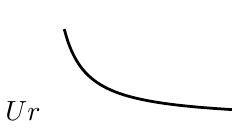
\begin{tikzpicture}\gaxesPN{$U$}{$r$}
    \draw[line width=1pt, domain=0.3:2.5, samples=50, smooth] plot (\x, {0.35/\x});
  \end{tikzpicture}}
  {%
  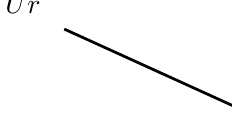
\begin{tikzpicture}\gaxesPN{$U$}{$r$}
    \draw[line width=1pt] (0.3,-0.2) -- (2.5,-1.2);
  \end{tikzpicture}}
  {%
  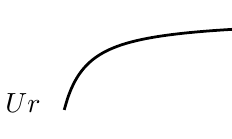
\begin{tikzpicture}\gaxesPN{$U$}{$r$}
    \draw[line width=1pt, domain=0.3:2.5, samples=50, smooth] plot (\x, {1.2-0.35/\x});
  \end{tikzpicture}}
  {%
  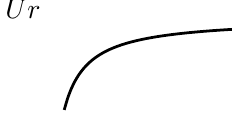
\begin{tikzpicture}\gaxesPN{$U$}{$r$}
    \draw[line width=1pt, domain=0.3:2.5, samples=50, smooth] plot (\x, {-0.35/\x});
  \end{tikzpicture}}
\end{quizq}

% ---- Q65 (escape velocity from the Moon)
\Needspace{12\baselineskip}
\begin{quizq}{}
The Moon has a mass of \qty{7.35e22}{kg} and a radius of \qty{1.74e6}{m}. What is the escape velocity
from the surface of the Moon?
\opts{\qty{1.68e3}{m.s^{-1}}}{\qty{2.37e3}{m.s^{-1}}}{\qty{7.51e4}{m.s^{-1}}}{\qty{5.64e6}{m.s^{-1}}}
\end{quizq}

% ---- Q66 (escape velocity with 4 times the mass)
\Needspace{12\baselineskip}
\begin{quizq}{}
The escape velocity from Earth's surface is \qty{11.2}{km.s^{-1}}. A planet has 4 times the mass of
Earth and the same radius as Earth.

What is the escape velocity from the surface of this planet?
\opts{\qty{5.6}{km.s^{-1}}}{\qty{11.2}{km.s^{-1}}}{\qty{22.4}{km.s^{-1}}}{\qty{44.8}{km.s^{-1}}}
\end{quizq}

% ---- Q67 (escape velocity statement)
\Needspace{14\baselineskip}
\begin{quizq}{}
Which statement about the escape velocity from a planet is correct?
\opts{It is greater for a rocket with a greater mass.}
  {It applies only when the object is launched vertically upwards.}
  {It is equal to the speed needed for a circular orbit at the same height.}
  {It is smaller at a greater distance from the centre of the planet.}
\end{quizq}

% ---- Q68 (energy to move a satellite from LEO to GEO)
\Needspace{14\baselineskip}
\begin{quizq}{}
A \qty{1000}{kg} satellite is moved from a circular orbit at an altitude of \qty{400}{km} to a
geostationary orbit of radius \qty{4.23e7}{m}. The total energy of a satellite in a circular orbit is
$E = -\dfrac{GMm}{2r}$.

What is the minimum energy that must be supplied to the satellite?
\opts{\qty{4.7e9}{J}}{\qty{2.5e10}{J}}{\qty{3.0e10}{J}}{\qty{5.0e10}{J}}
\end{quizq}

% ---- Q69 (point of zero net force if the Moon were heavier)
\Needspace{15\baselineskip}
\begin{quizq}{}
On the line between Earth and the Moon there is a point where the net gravitational force on a
spacecraft is zero.

If the Moon's mass were 4 times bigger (with everything else the same), where would this point be?
\opts{Closer to the Moon than before}{In the same place as before}{There would no longer be such a
  point}{Closer to Earth than before}
\end{quizq}

% ---- Q70 (ratio of centripetal accelerations)
\Needspace{13\baselineskip}
\begin{quizq}{}
Satellites P and Q move in circular orbits around Earth. The orbital radius of Q is 4 times the
orbital radius of P.

What is the ratio $\dfrac{\text{centripetal acceleration of P}}{\text{centripetal acceleration of Q}}$?
\opts{2}{4}{8}{16}
\end{quizq}

% ---- Q71 (orbital speed of a geostationary satellite)
\Needspace{11\baselineskip}
\begin{quizq}{}
What is the orbital speed of a geostationary satellite (period 24.0 hours)?
\opts{\qty{4.6e2}{m.s^{-1}}}{\qty{3.1e3}{m.s^{-1}}}{\qty{7.7e3}{m.s^{-1}}}{\qty{1.1e4}{m.s^{-1}}}
\end{quizq}

% ---- Q72 (U and E from the kinetic energy)
\Needspace{22\baselineskip}
\begin{quizq}{}
A satellite in a circular orbit has a kinetic energy of \qty{3.0e9}{J}.

Which row of the table correctly gives its gravitational potential energy and its total energy?
\begin{center}
  \renewcommand\arraystretch{1.7}
  \begin{tabular}{@{}p{10mm}|>{\centering\arraybackslash}p{55mm}|>{\centering\arraybackslash}p{40mm}|}
    \cline{2-3}
    & \textit{Gravitational potential energy} & \textit{Total energy}\\ \cline{2-3}
    A. & \qty{-3.0e9}{J} & \qty{0}{J}\\ \cline{2-3}
    B. & \qty{-6.0e9}{J} & \qty[retain-explicit-plus]{+3.0e9}{J}\\ \cline{2-3}
    C. & \qty{-1.5e9}{J} & \qty[retain-explicit-plus]{+1.5e9}{J}\\ \cline{2-3}
    D. & \qty{-6.0e9}{J} & \qty{-3.0e9}{J}\\ \cline{2-3}
  \end{tabular}
\end{center}
\end{quizq}
